Cílem práce bylo navrhnout a implementovat webovou aplikaci umožňující stažení 3D modelů dílů LEGO. Tento cíl byl úspěšně naplněn včetně zveřejnění aplikace do sítě internet. 

V~rešeršní části práce byly nejprve představeny služby poskytující data o~sou\-část\-kách a stavebnicích LEGO, dále byly představeny programy pro převod formátu LDraw na formát \textit{STL}.

Na základě rešerše byl následně proveden návrh architektury aplikace a uži\-va\-tel\-ské\-ho rozhraní, ze kterého bylo vycházeno při samotné implementaci. 

Instance aplikace je nasazena a připravena k~používání na adrese \url{http://printabrick.org}. 

Zdrojový kód aplikace je zveřejněn pod open-source licencí \gls{GPLv2} \autocite{GPLv2} a veřejně dostupný na \url{https://github.com/hubnedav/PrintABrick}.

\begin{figure}[htbp]
    \centering
    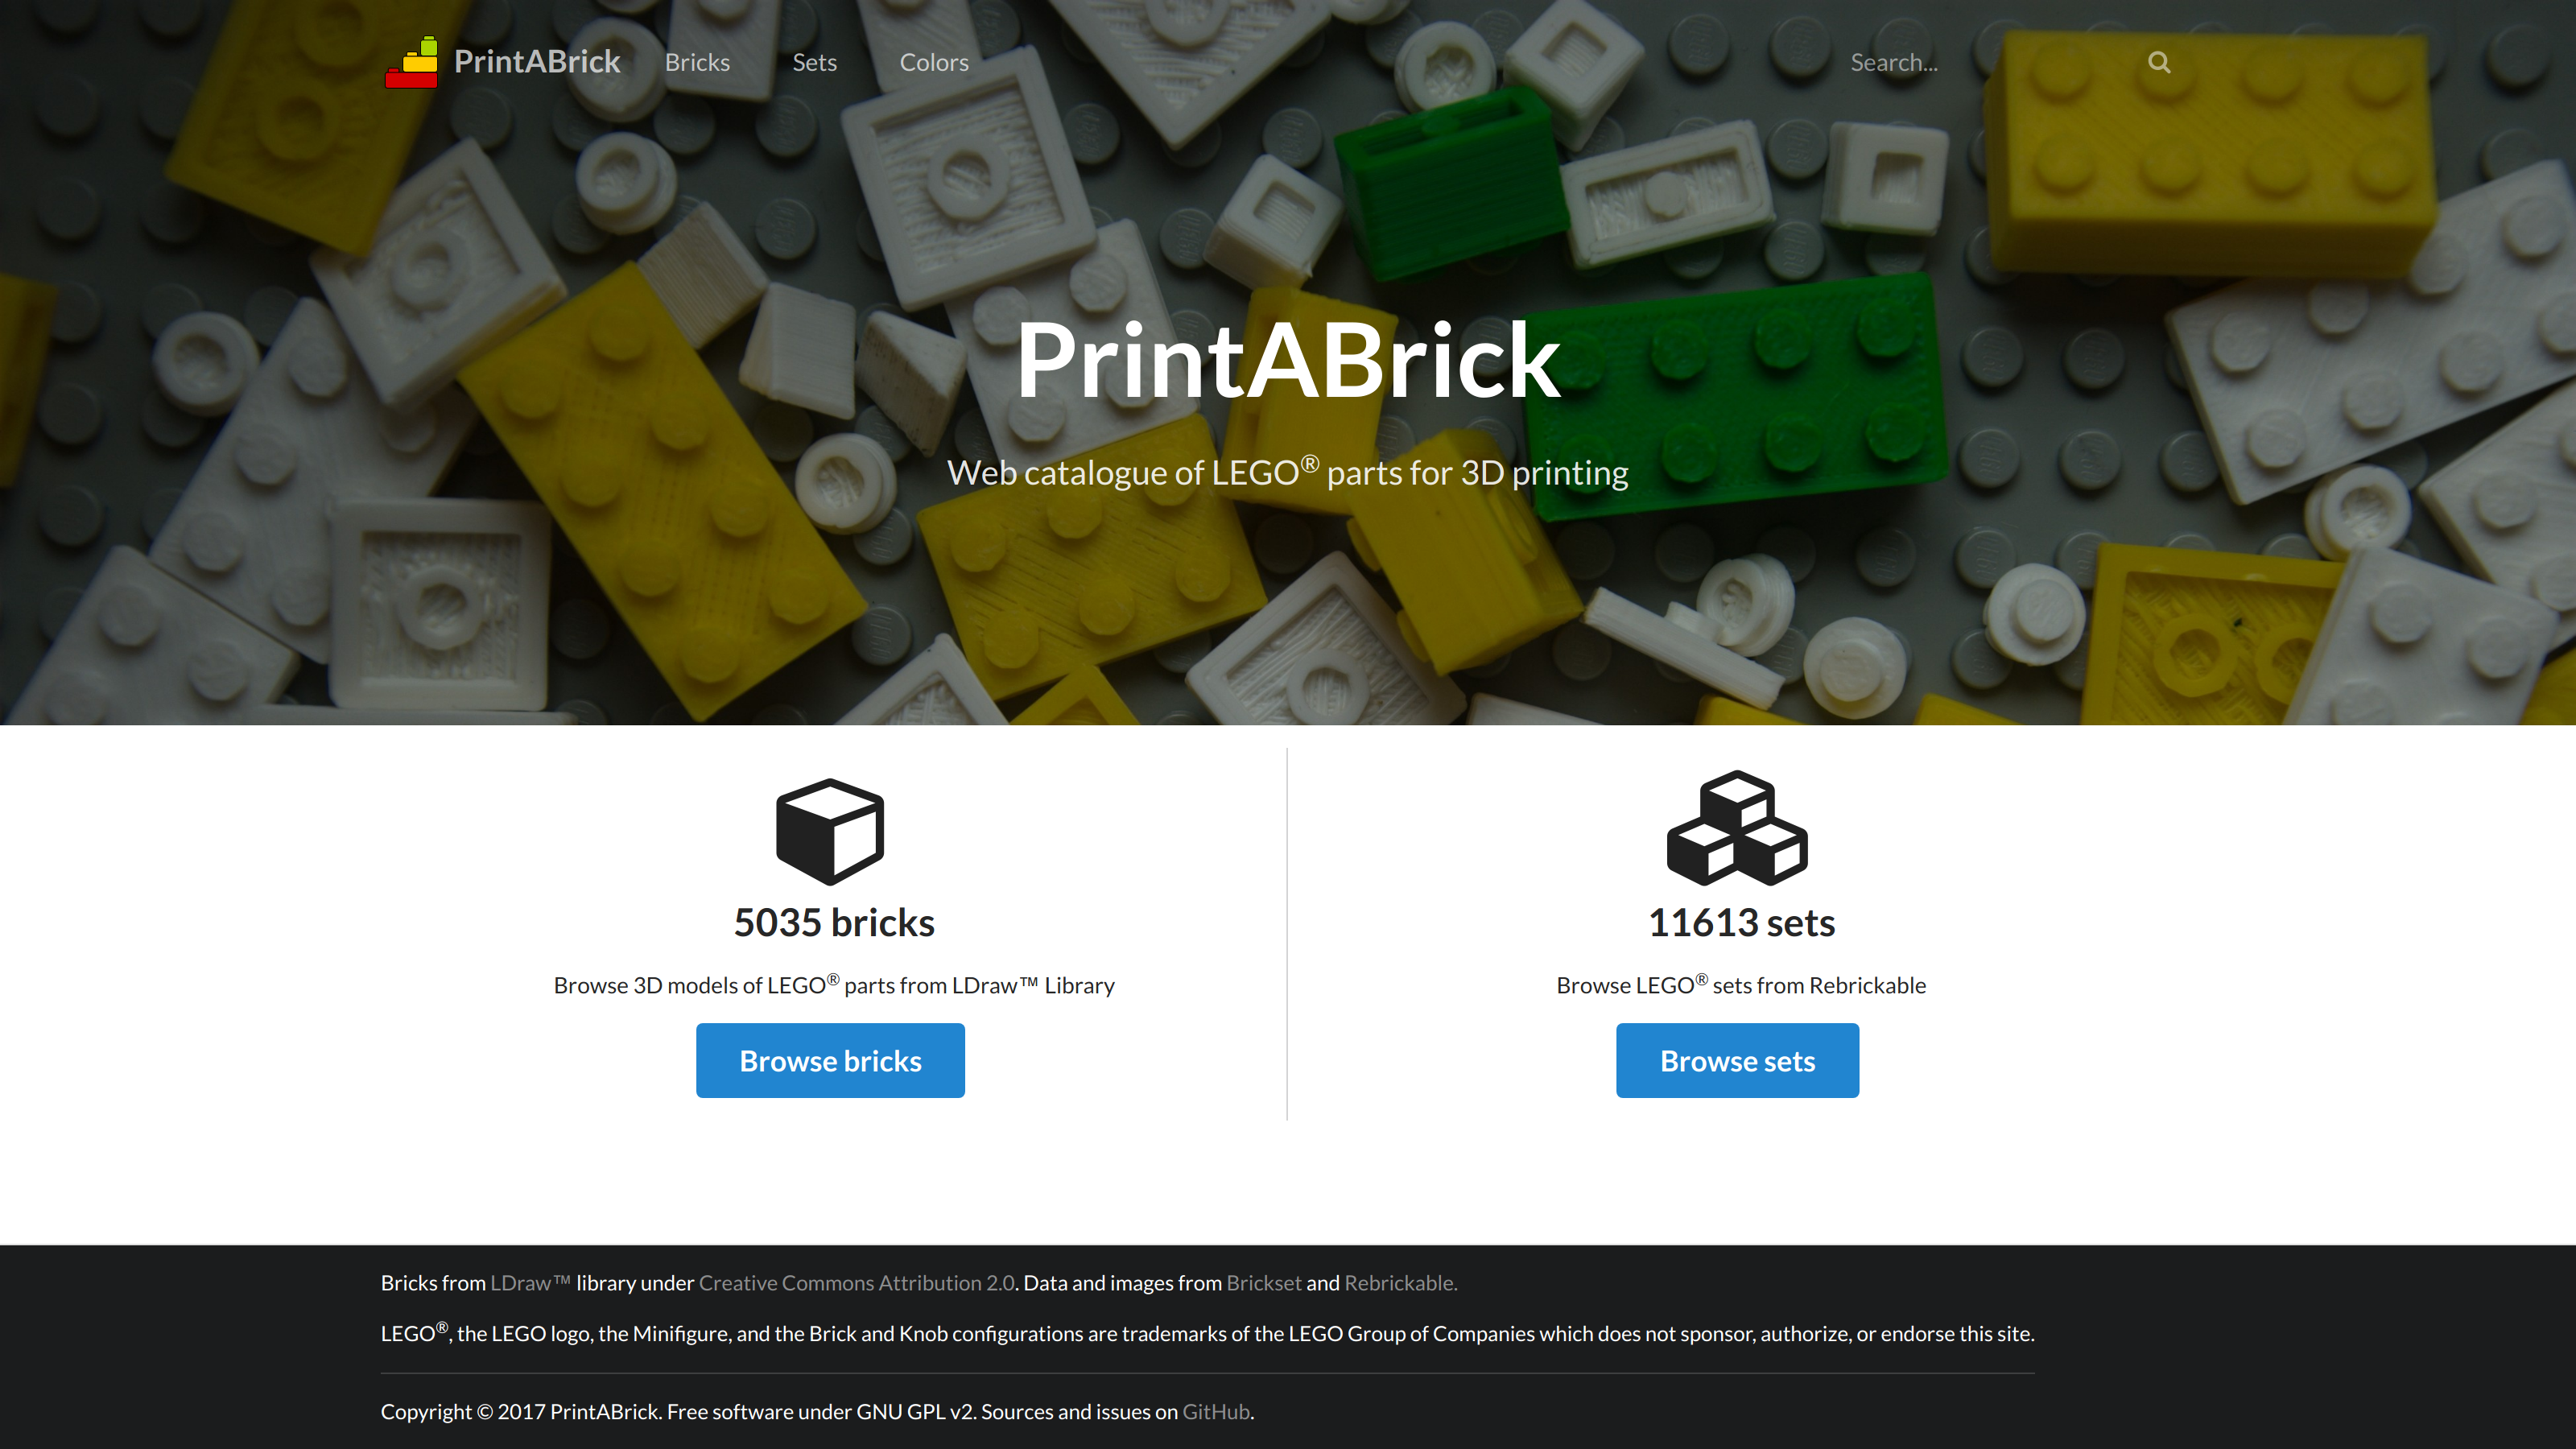
\includegraphics[width=\textwidth,height=\textheight,keepaspectratio]{images/screenshot-homepage.png}
    \caption{Snímek obrazovky – domovská stránka\label{facebook-share}}
\end{figure}

\begin{figure}[htbp]
    \centering
    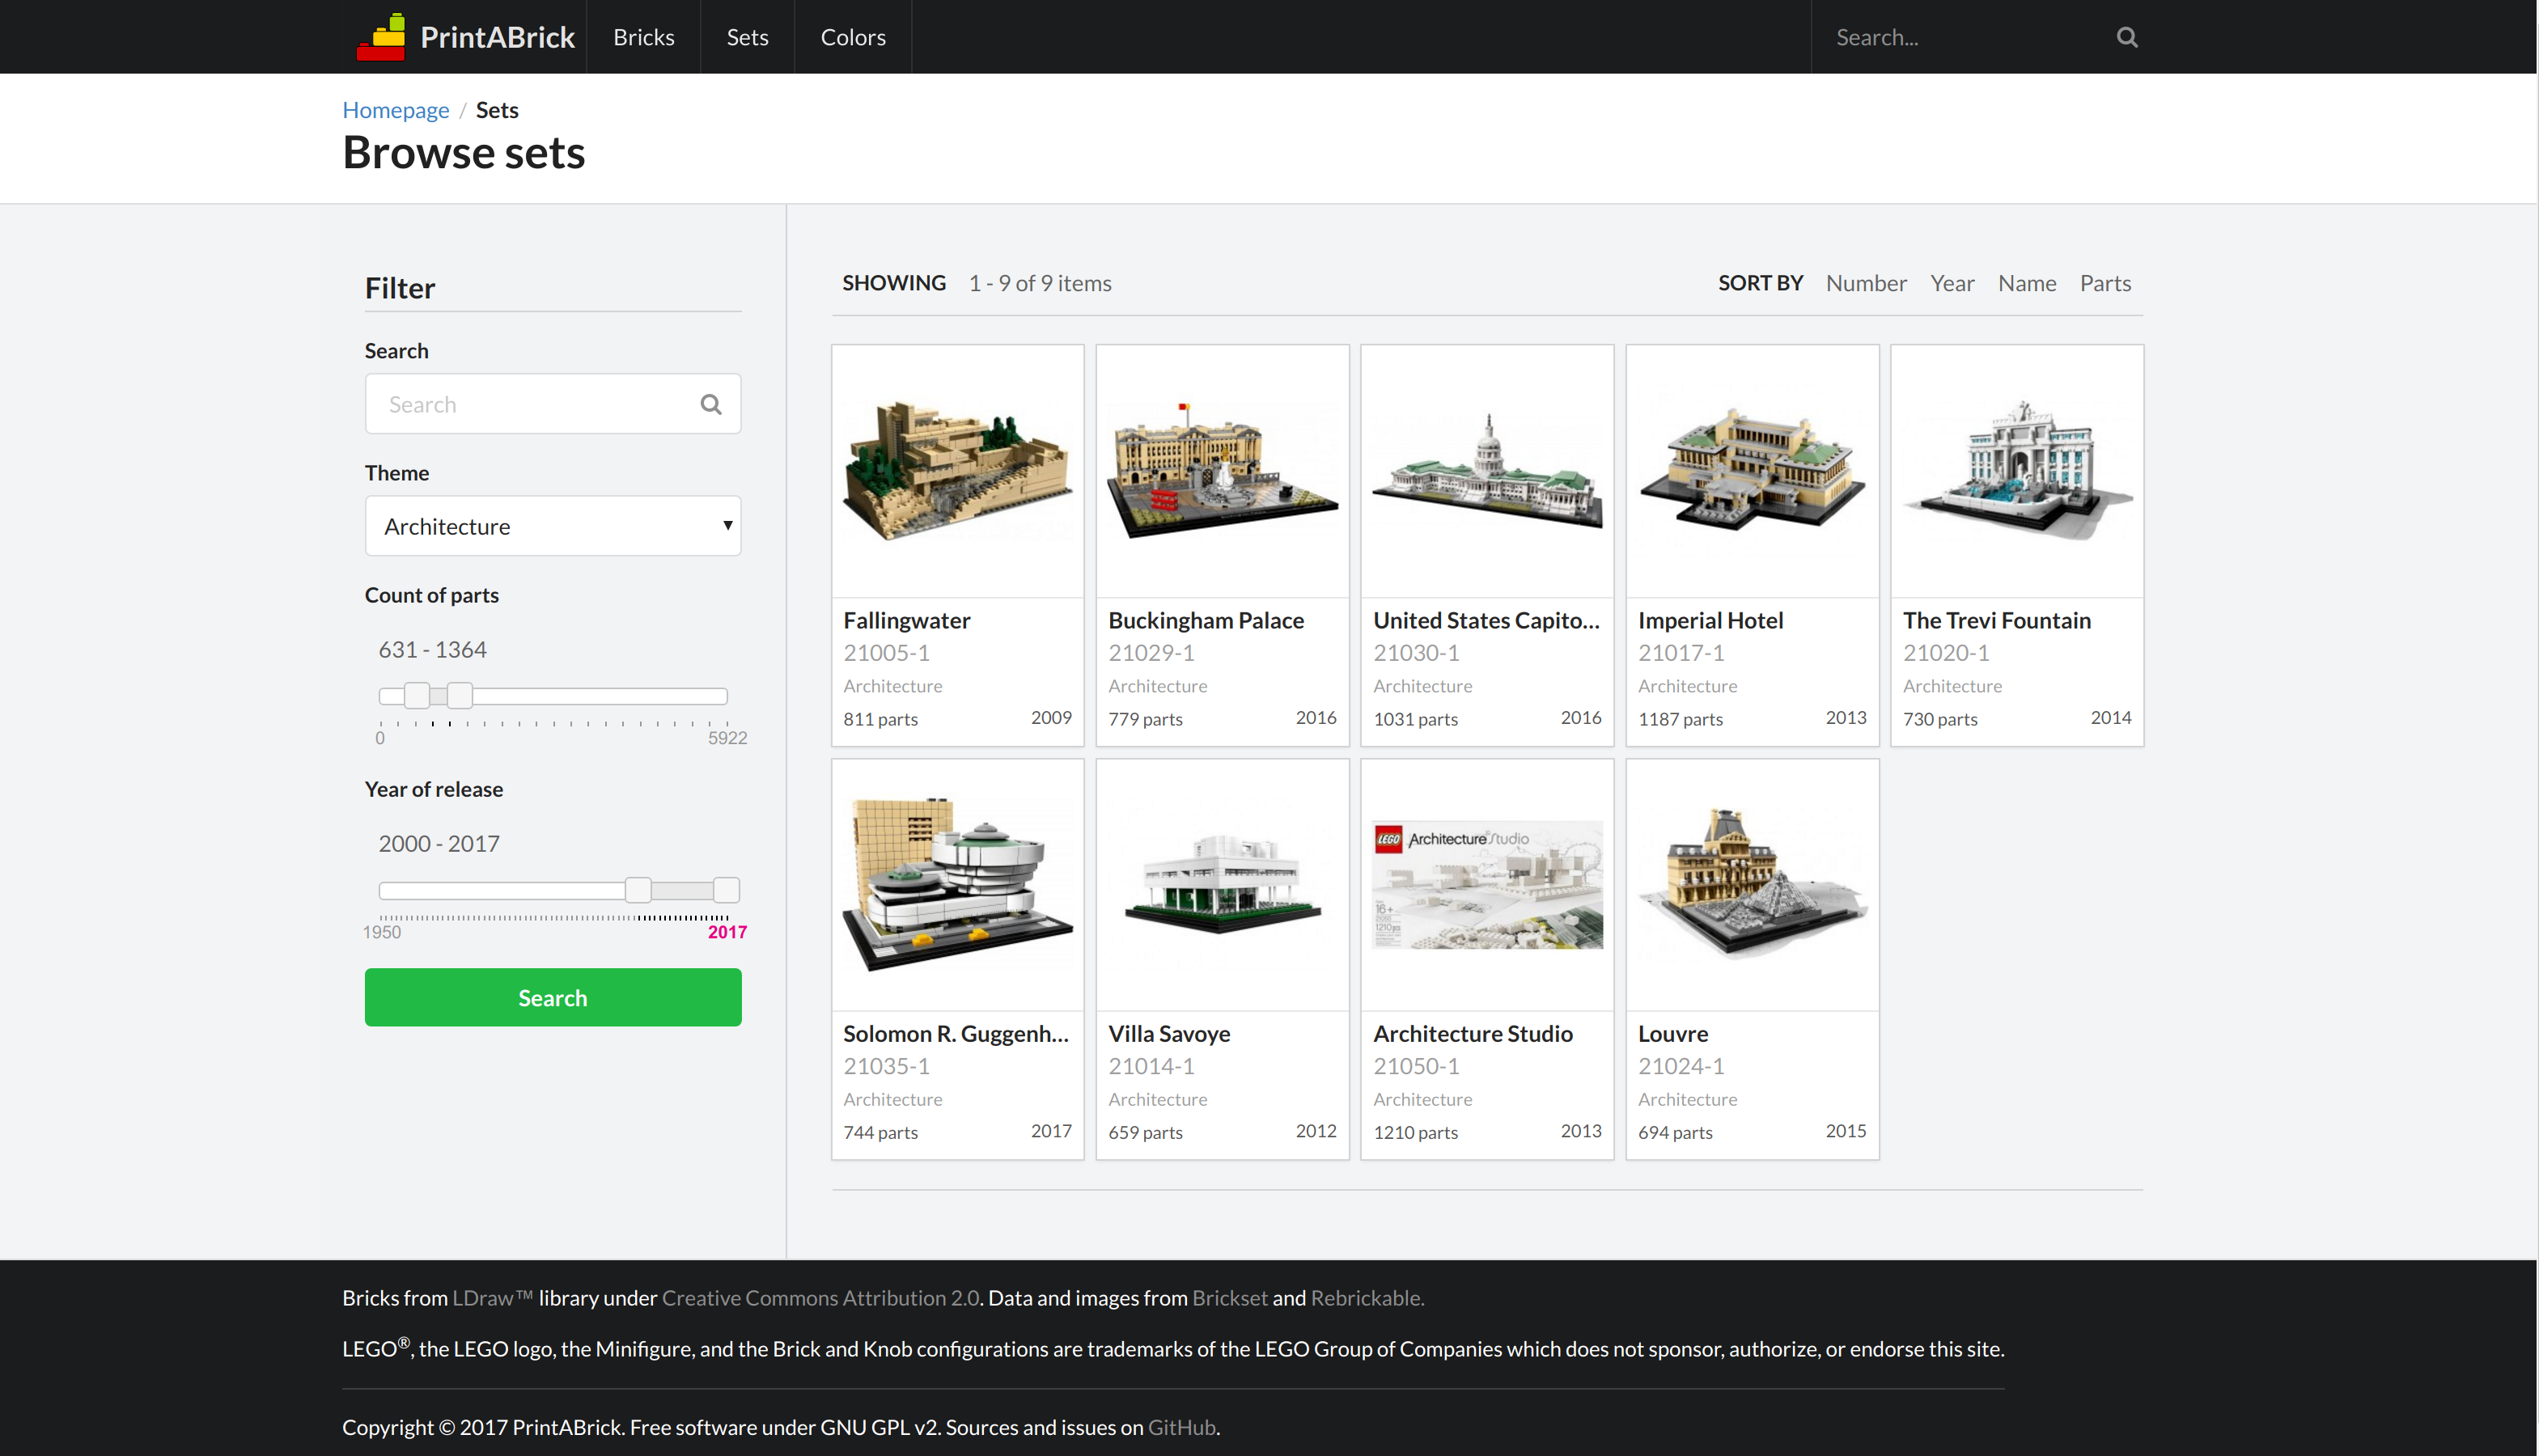
\includegraphics[width=\textwidth,height=\textheight,keepaspectratio]{images/screenshot-sets.png}
    \caption{Snímek obrazovky – výpis stavebnic\label{facebook-share}}
\end{figure}

\subsubsection*{Možnosti dalšího rozvoje}\label{moznosti-dalsiho-rozvoje}

V~rámci dalšího rozvoje aplikace vidím následující možnosti:
\begin{itemize}
    \item výpočet odhadu množství materiálu potřebného k~tisku,
    \item využití uživatelských dat pro správu sbírek přes API Rebrickable,
    \item provedení uživatelského testování s~následnou opravou zjištěných závad.
\end{itemize} 
